% PRL look and style (easy on the eyes)
\documentclass[aps,pre,twocolumn,superscriptaddress,nofootinbib]{revtex4}
% Two-column style (for submission/review/editing)
%\documentclass[aps,preprint,prl,superscriptaddress,showpacs]{revtex4}

\usepackage{palatino}
\usepackage{amsmath}
\usepackage{amssymb}
\usepackage{graphicx}
\usepackage{dcolumn}
\usepackage{boxedminipage}
\usepackage{verbatim}
\usepackage[colorlinks=true,citecolor=blue,linkcolor=blue]{hyperref}

% The figures are in a figures/ subdirectory.
\graphicspath{{figures/}}

%\bibliographystyle{apsrevlong}
\bibliographystyle{apsrev}

% italicized boldface for math (e.g. vectors)
\newcommand{\bfv}[1]{{\mbox{\boldmath{$#1$}}}}
% non-italicized boldface for math (e.g. matrices)
\newcommand{\bfm}[1]{{\bf #1}}          

%\newcommand{\bfm}[1]{{\mbox{\boldmath{$#1$}}}}
%\newcommand{\bfm}[1]{{\bf #1}}
\newcommand{\expect}[1]{\left \langle #1 \right \rangle}                % <.> for denoting expectations over realizations of an experiment or thermal averages

% vectors
\newcommand{\x}{\bfv{x}}
\newcommand{\y}{\bfv{y}}
\newcommand{\f}{\bfv{f}}

\newcommand{\bfc}{\bfm{c}}
\newcommand{\hatf}{\hat{f}}

\newcommand{\bTheta}{\bfm{\Theta}}
\newcommand{\btheta}{\bfm{\theta}}
\newcommand{\bhatf}{\bfm{\hat{f}}}
\newcommand{\Cov}[1] {\mathrm{cov}\left( #1 \right)}
\newcommand{\Ept}[1] {{\mathrm E}\left[ #1 \right]}
\newcommand{\Eptk}[2] {{\mathrm E}_{#1}\left[ #2\right]}
\newcommand{\T}{\mathrm{T}}                                % T used in matrix transpose

% Commands to force LaTeX to put two figures on a page:
\renewcommand{\textfraction}{0.05}
\renewcommand{\topfraction}{0.95}
\renewcommand{\bottomfraction}{0.95}
\renewcommand{\floatpagefraction}{0.35}
\setcounter{totalnumber}{5}

%% DOCUMENT %%%%%%%%%%%%%%%%%%%%%%%%%%%%%%%%%%%%%%%%%%%%%%%%%%%%%%%%%%%%%%%%%%%%
\begin{document}

%% TITLE %%%%%%%%%%%%%%%%%%%%%%%%%%%%%%%%%%%%%%%%%%%%%%%%%%%%%%%%%%%%%%%%%%%%
\title{Comment on ``Bayesian estimates of free energies from nonequilibrium work data in the presence of instrument noise''}

\author{John D. Chodera}
 \email{jchodera@stanford.edu}
 \thanks{Author to whom correspondence should be addressed.}
 \affiliation{Department of Chemistry, Stanford University, Stanford, CA 94305, USA}
\author{David D. L. Minh}
 \email{daveminh@gmail.com}
 \affiliation{Laboratory of Chemical Physics, NIDDK, National Institutes of Health, Bethesda, Maryland 20892, USA}
\author{Michael R. Shirts}
 \email{mrshirts@gmail.com}
 \affiliation{Department of Chemical Engineering, University of Virginia, Charlottesville, VA 22904, USA}

\date{\today}

%%%%%%%%%%%%%%%%%%%%%%%%%%%%%%%%%%%%%%%%%%%%%%%%%%%%%%%%%%%%%%%%%%%%%%%%%%%%%%%%%%%%%%%%%%%%%%%%%%%%%%
% NO ABSTRACT
%%%%%%%%%%%%%%%%%%%%%%%%%%%%%%%%%%%%%%%%%%%%%%%%%%%%%%%%%%%%%%%%%%%%%%%%%%%%%%%%%%%%%%%%%%%%%%%%%%%%%%
%\begin{abstract}
%\end{abstract}

\maketitle

%%%%%%%%%%%%%%%%%%%%%%%%%%%%%%%%%%%%%%%%%%%%%%%%%%%%%%%%%%%%%%%%%%%%%%%%%%%%%%%%%%%%%%%%%%%%%%%%%%%%%%
% BODY
%%%%%%%%%%%%%%%%%%%%%%%%%%%%%%%%%%%%%%%%%%%%%%%%%%%%%%%%%%%%%%%%%%%%%%%%%%%%%%%%%%%%%%%%%%%%%%%%%%%%%%

The development of methods to estimate free energy differences from nonequilibrium work measurements remains an active area of research.  
Recently, Maragakis et al.~presented a new Bayesian scheme for the analysis of single-molecule pulling data in the presence of instrument noise~\cite{maragakis:jcp:2008:bayesian-bar}.
In principle, Bayesian methods provide a powerful tool for assessing the confidence in an estimate, thereby guiding experimentalists in deciding how much data need be collected.  
However, we believe that a word of caution is necessary, as this method can produce misleading estimates of the uncertainty when improperly applied.

Our concern lies with the posterior distribution for the free energy estimate $\Delta F_\Lambda$ given measured work values $W$ and protocols $\Lambda$ (forward or reverse measurements) in the absence of measurement error, which forms the core of proposed scheme~\cite{maragakis:jcp:2008:bayesian-bar}:
\begin{eqnarray}
P(\Delta F_{\Lambda} | W_n,\Lambda) &\propto& P(W, \Lambda | \Delta F_{\Lambda}) \, P(\Delta F_{\Lambda}) \nonumber \\
&\propto& \prod_{n=1}^N f(\beta W_n - \beta \Delta F_{\Lambda_n} + M_{\Lambda_n}) \label{equation:posterior}
\end{eqnarray}
In this expression, $\beta$ is the inverse temperature, $f(x) = (1+e^{-x})^{-1}$ is the standard logistic function, and  $M_\Lambda = \ln (N_\Lambda / N_{\tilde{\Lambda}})$ is the log ratio of the number of forward and reverse work measurements.
The method can be thought of as a Bayesian extension to the Bennett acceptance ratio (BAR)~\cite{bennett:j-comput-phys:1976:bar}, and will henceforth be referred to as BBAR for brevity.

% JDC: Maybe we should use F and R instead of this Lambda business?  Would that make things more readable?

Though derivation of the Bayesian~\cite{maragakis:jcp:2008:bayesian-bar} and maximum likelihood~\cite{shirts:prl:2003:bar,maragakis:prl:2006:pbar} variants differ slightly, both contain an essential step such as the one used to compute $P(W, \Lambda | \Delta F)$ from known quantities:
\begin{eqnarray}
\frac{P(+W, \Lambda | \Delta F_{\Lambda})}{P(-W, \tilde{\Lambda} | \Delta F_{\tilde{\Lambda}})} &=& \frac{ P(+W | \Lambda, \Delta F_{\Lambda})}{P(-W | \tilde{\Lambda}, \Delta F_{\tilde{\Lambda}})} \cdot \frac{P(\Lambda | \Delta F_{\Lambda})}{P(\tilde{\Lambda} | \Delta F_{\tilde{\Lambda}})} \label{equation:likelihood-ratio}
\end{eqnarray}
The Crooks fluctuation theorem~\cite{crooks:pre:1999:cft} can be used to evaluate the first ratio, and the second ratio --- the relative probability of forward measurements $\Lambda$ over reverse measurements $\tilde{\Lambda}$ --- is evaluated as $N_\Lambda / N_{\tilde{\Lambda}}$.
Together with the assumption that $P(+W | \Lambda, \Delta F_{\Lambda}) + P(-W | \tilde{\Lambda}, \Delta F_{\tilde{\Lambda}})$ is constant --- a necessary assumption in order to provide a prior on the work distribution --- Eq.~\ref{equation:posterior} is obtained.

We point out two features of the Bayesian posterior (Eq.~\ref{equation:posterior}).
First, if either $N_\Lambda$ or $N_{\tilde{\Lambda}}$ are zero --- only work measurements along one protocol (but not its reverse) are available --- the posterior is unnormalizable, and no estimate is produced, only a soft bound~\footnote{There is also the problem that $M_\Lambda$ may be undefined, but Maragakis et al.~propose the modified definition $M_\Lambda = \ln (N_\Lambda + 1) / (N_{\tilde{\Lambda}} + 1)$ as a way to avoid this~\cite{maragakis:jcp:2008:bayesian-bar}.}.
This need not be the case: A recent multistate extension of BAR~\cite{shirts:jcp:2008:mbar} provides both an estimator and an estimate of the statistical uncertainty (through an asymptotic variance estimate) in this case as well.
It may be possible to construct a modified posterior that also furnishes a well-defined estimate for this situation.

The second issue provides a caution for both BBAR and methods based on the likelihood approach lies in the separation of work measurements from their protocol to produce the ratio $P(\Lambda | \Delta F_\Lambda) / P(\tilde{\Lambda} | \Delta F_{\tilde{\Lambda}})$, evaluated as $N_\Lambda / N_{\tilde{\Lambda}}$.
Most experiments are not conducted with a fixed \emph{probability} of recording forward and reverse measurements, which would allow the actual number of samples in each direction to vary, but a fixed \emph{number} of measurements in each direction.
Because of this difference, Shirts et al.~\cite{shirts:prl:2003:bar} were forced to employ a correction term~\cite{anderson.biometrika:1972:logistic-discrimination} that reduced the variance by $- (N_{\Lambda}^{-1} + N_{\tilde{\Lambda}}^{-1})$ in order to produce an estimate of the uncertainty that agreed with the original derivation by Bennett~\cite{bennett:j-comput-phys:1976:bar}.

Only much later was it appreciated that Geyer had earlier proposed a similar likelihood approach, framing the problem as ``reverse logistic regression''~\cite{geyer:techrep:1994:reverse-logistic-regression}.
Geyer's method suffered from the same problem, in that the uncorrected asymptotic variance of the likelihood function gives an overestimate of the statistical uncertainty, for reasons elegantly explained by Kong et al.~\cite{kong:j-r-stat-soc-b:2003:bridge-sampling}.
While the estimators are asymptotically unbiased for both types of experiments (fixed-number and fixed-probability), there is a clear difference in the asymptotic variance of the estimator between these two types of experiments~\cite{kong:j-r-stat-soc-b:2003:bridge-sampling}.
It is reasonable to ask, therefore, what practical impact this difference has on BBAR, and under what conditions we might find the posterior to be unreliable.

% Coin-flip inference example.
\begin{figure}[htb]
  \begin{center}
    \resizebox{\columnwidth}{!}{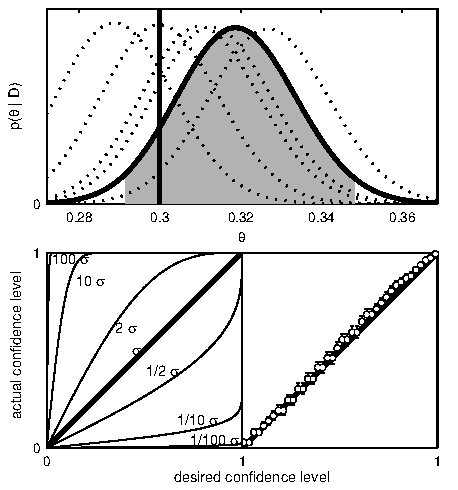
\includegraphics{coinflip}}
  \end{center}
  \caption{{\bf Testing the posterior for inference of a biased coin flip experiment.}
  \emph{Top:} Posterior distribution for inferring the probability of heads, $\theta$, for a biased coin from an sequence of $N = 1000$ coin flips (dark line) with 95\% symmetric confidence interval about the mean (shaded area).
  The true probability of heads is 0.3 (vertical thick line).
  Posteriors from five different experiments are shown as dotted lines.
  \emph{Bottom left:} Desired and actual confidence levels for an idealized normal posterior distribution that either overestimates (upper left curves) or underestimates (bottom right curves) the true posterior variance by different degrees.
  \emph{Bottom right:} Desired and actual confidence levels for the Binomial-Beta posterior for the coin flip problem depicted in upper panel.   Error bars show 95\% confidence intervals estimates from 1000 independent experimental trials.
  For inference, we use a likelihood function such that the observed number of heads is $N_H | \theta \sim \mathrm{Binomial}(N_H, N, \theta)$ and conjugate Jeffreys prior~\cite{jeffreys:proc-royal-soc-london:1946:jeffreys-prior,goyal:aip-proceedings:2005:jeffreys-prior} $\theta \sim \mathrm{Beta}(1/2, 1/2)$ which produces posterior $\theta | N_H \sim \mathrm{Beta}(N_H + 1/2, N_T + 1/2)$ along with constraint $N_H + N_T = N$.
  }
  \label{figure:biased-coin}
\end{figure}

How can we test a Bayesian posterior distribution? 
One of the more powerful features of a Bayesian model is its ability to provide confidence intervals that correctly reflect the level of certainty that the true value will lie within in.
For example, if the experiment were to be repeated many times, the true value of the parameter being estimated should fall within the confidence interval for a 95\% confidence level 95\% of the time.
As an illustrative example, consider a biased coin where the probability of turning heads is $\theta$.
From an observed sample of N coin flips, we can estimate $\theta$ using a Binomial model for the number of coin flips that turn up heads and a conjugate Beta Jeffreys prior~\cite{jeffreys:proc-royal-soc-london:1946:jeffreys-prior,goyal:aip-proceedings:2005:jeffreys-prior}.
Each time we run experiment, we get a different posterior estimate for $\theta$, and a different confidence interval (Figure \ref{figure:biased-coin}, top).
If we run many trials and record what fraction of the time the true (unknown) value of $\theta$ falls within the confidence interval estimated from that trial, we can see if our model is correct.
If correct, the observed confidence level should match the desired confidence level (Figure \ref{figure:biased-coin}, bottom right).
Deviation from parity means that the posterior is either two broad or too narrow, and that the statistical uncertainty is being either over- or underestimated (Figure \ref{figure:biased-coin}, bottom left).

% Test of BBAR.
\begin{figure}[htb]
  \begin{center}
    \resizebox{\columnwidth}{!}{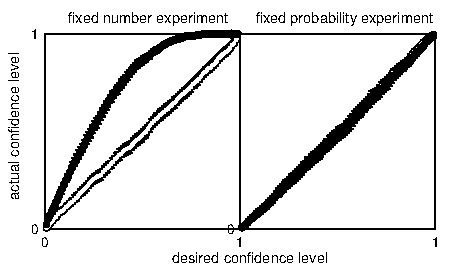
\includegraphics{bbar-gaussian-sigma=1-10-10}}
    \resizebox{\columnwidth}{!}{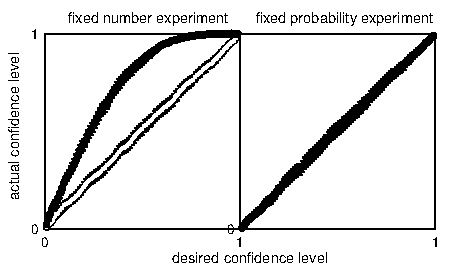
\includegraphics{bbar-gaussian-sigma=1-100-100}}
    \resizebox{\columnwidth}{!}{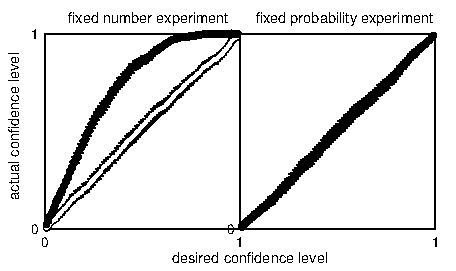
\includegraphics{bbar-gaussian-sigma=1-1000-1000}}
  \end{center}
  \caption{{\bf Testing the posterior for Bayesian BAR.}
  \emph{Left:} Actual confidence levels for BBAR (filled circles) and BAR-FN (solid circles) evaluated for replications of an experiment containing a \emph{fixed number} of 10 (top), 100 (middle), or 1000 (bottom) work measurements in each direction. 
  \emph{Right:} Actual confidence levels for \emph{fixed probability} case comparing BBAR (filled circles) and BAR-FP (solid circles).
  Error bars show 95\% confidence intervals estimated from 1000 independent experimental trials.
%  Work measurements were obtained from simultaneous switching between two harmonic oscillators defined by spring constants $\beta K = \{1, 4\}$ with minima displaced by $\Delta x = 1.5$.
  Work measurements were obtained from a model with Gaussian forward work distribution of unit mean and variance; the reverse work distribution is fully determined from the forward distribution by the Crooks fluctuation theorem~\cite{crooks:pre:1999:cft}.
  Tests with a system of displaced one-dimensional harmonic oscillators showed similar behavior.
  }
  \label{figure:bbar-test}
\end{figure}

We tested the BBAR posterior in the same way on a two-state system with Gaussian work distributions (Figure \ref{figure:bbar-test}).
We compared the behavior with the asymptotic variance estimates of standard BAR~\cite{bennett:j-comput-phys:1976:bar,shirts:prl:2003:bar,shirts:jcp:2008:mbar}, which effectively assumes a normal posterior, either with the correction for fixed-number (BAR-FN) or without the correction, which would be appropriate for fixed-probability experiments (BAR-FP).
We find that, under a variety of conditions, BBAR significantly overestimates the uncertainty in experiments where a fixed number of forward and reverse work measurements are made, while BAR-FN accurately estimates the confidence intervals (Figure \ref{figure:bbar-test}, left column).
This behavior persists for both small (top) and large (bottom) numbers of samples.
If instead the experiment is run where forward or reverse measurements are selected according to a fixed probability, we see that BBAR correctly estimates the true confidence intervals, as does BAR-FP (Figure \ref{figure:bbar-test}, right column).

In light of these results, we make the following recommendations, until such time as additional theory work can produce a variant of BBAR appropriate for the fixed-number experiment.
(1) Practitioners of simulation or experiment should incorporate a fixed probability of forward or reverse measurement into their experimental design, or post-process the data by picking a subset of data from the pool of measurements with fixed probability in estimating the error in the estimate (which can still be produced from the entire dataset without concern).
(2) Theorists wishing to produce estimators based on BBAR should exercise caution that their experimental design corresponds to the fixed-probability, rather than the fixed-number, situation, unless a large upper bound on the uncertainty can be tolerated.

%%%%%%%%%%%%%%%%%%%%%%%%%%%%%%%%%%%%%%%%%%%%%%%%%%%%%%%%%%%%%%%%%%%%%%%%%%%%%%%%%%%%%%%%%%%%%%%%%%%%%%
% ACKNOWLEDGMENTS
%%%%%%%%%%%%%%%%%%%%%%%%%%%%%%%%%%%%%%%%%%%%%%%%%%%%%%%%%%%%%%%%%%%%%%%%%%%%%%%%%%%%%%%%%%%%%%%%%%%%%%
\begin{acknowledgments}
The authors thank Gavin E. Crooks (Lawrence Berkeley Natl.~Lab.)~and Paul Maragakis (D.~E.~Shaw Research) for enlightening discussions of their work.
JDC acknowledges support through an NSF grant for Cyberinfrastructure (NSF CHE-0535616) through Vijay S. Pande.
\end{acknowledgments}

%%%%%%%%%%%%%%%%%%%%%%%%%%%%%%%%%%%%%%%%%%%%%%%%%%%%%%%%%%%%%%%%%%%%%%%%%%%%%%%%%%%%%%%%%%%%%%%%%%%%%%
% BIBLIOGRAPHY
%%%%%%%%%%%%%%%%%%%%%%%%%%%%%%%%%%%%%%%%%%%%%%%%%%%%%%%%%%%%%%%%%%%%%%%%%%%%%%%%%%%%%%%%%%%%%%%%%%%%%%
\bibliographystyle{prsty} 
\bibliography{comment-on-bayesian-BAR}

\end{document}